%%
%% Automatically generated ptex2tex (extended LaTeX) file
%% from Doconce source
%% http://code.google.com/p/doconce/
%%




%-------------------------- begin preamble --------------------------
\documentclass[twoside]{article}



\usepackage{relsize,epsfig,makeidx,amsmath,amsfonts}
\usepackage[latin1]{inputenc}
\usepackage{minted} % packages needed for verbatim environments


% Hyperlinks in PDF:
\usepackage[%
    colorlinks=true,
    linkcolor=black,
    %linkcolor=blue,
    citecolor=black,
    filecolor=black,
    %filecolor=blue,
    urlcolor=black,
    pdfmenubar=true,
    pdftoolbar=true,
    urlcolor=black,
    %urlcolor=blue,
    bookmarksdepth=3   % Uncomment (and tweak) for PDF bookmarks with more levels than the TOC
            ]{hyperref}
%\hyperbaseurl{}   % hyperlinks are relative to this root

% Tricks for having figures close to where they are defined:
% 1. define less restrictive rules for where to put figures
\setcounter{topnumber}{2}
\setcounter{bottomnumber}{2}
\setcounter{totalnumber}{4}
\renewcommand{\topfraction}{0.85}
\renewcommand{\bottomfraction}{0.85}
\renewcommand{\textfraction}{0.15}
\renewcommand{\floatpagefraction}{0.7}
% 2. ensure all figures are flushed before next section
\usepackage[section]{placeins}
% 3. enable begin{figure}[H] (often leads to ugly pagebreaks)
%\usepackage{float}\restylefloat{figure}

\newcommand{\inlinecomment}[2]{  ({\bf #1}: \emph{#2})  }
%\newcommand{\inlinecomment}[2]{}  % turn off inline comments

% insert custom LaTeX commands...

\makeindex

\begin{document}
%-------------------------- end preamble --------------------------





% ----------------- title -------------------------

\begin{center}
{\LARGE\bf Experiments with Schemes for \\ [1.5mm] Exponential Decay}
\end{center}




% ----------------- author(s) -------------------------

\begin{center}
{\bf Hans Petter Langtangen${}^{1, 2}$ (\texttt{hpl@simula.no})} \\ [0mm]
\end{center}

\begin{center}
% List of all institutions:
\centerline{{\small ${}^1$Center for Biomedical Computing, Simula Research Laboratory}}
\centerline{{\small ${}^2$Department of Informatics, University of Oslo.}}
\end{center}
% ----------------- end author(s) -------------------------



% ----------------- date -------------------------


\begin{center}
August 20, 2012
\end{center}

\vspace{1cm}



\begin{abstract}
This report investigates the accuracy of three finite difference
schemes for the ordinary differential equation $u'=-au$ with the
aid of numerical experiments. Numerical artifacts are in particular
demonstrated.



\end{abstract}

\tableofcontents



% Section with multi-line equation.


\section{Mathematical problem}

\label{math:problem}

\index{model problem} \index{exponential decay}

We address the initial-value problem

\begin{align}
u'(t) &= -au(t), \quad t \in (0,T], \label{ode}\\
u(0)  &= I,                         \label{initial:value}
\end{align}
where $a$, $I$, and $T$ are prescribed parameters, and $u(t)$ is
the unknown function to be estimated. This mathematical model
is relevant for physical phenomena featuring exponential decay
in time.

% Section with single-line equation and a bullet list.


\section{Numerical solution method}

\label{numerical:problem}

\index{mesh in time} \index{$\theta$-rule} \index{numerical scheme}
\index{finite difference scheme}

We introduce a mesh in time with points $0= t_0< t_1 \cdots < t_N=T$.
For simplicity, we assume constant spacing $\Delta t$ between the
mesh points: $\Delta t = t_{n}-t_{n-1}$, $n=1,\ldots,N$. Let
$u^n$ be the numerical approximation to the exact solution at $t_n$.

The $\theta$-rule is used to solve (\ref{ode}) numerically:

\[
u^{n+1} = \frac{1 - (1-\theta) a\Delta t}{1 + \theta a\Delta t}u^n,
\]
for $n=0,1,\ldots,N-1$. This scheme corresponds to

\begin{itemize}
  \item The Forward Euler scheme when $\theta=0$

  \item The Backward Euler scheme when $\theta=1$

  \item The Crank-Nicolson scheme when $\theta=1/2$
% Section with computer code taken from a part of
% a file. The fromto: f@t syntax copies from the
% regular expression f up to the line, but not
% including, the regular expression t.
\end{itemize}

\noindent


\section{Implementation}

The numerical method is implemented in a Python function:

\begin{minted}[fontsize=\fontsize{9pt}{9pt},linenos=false,mathescape,baselinestretch=1.0,fontfamily=tt,xleftmargin=7mm]{python}
def theta_rule(I, a, T, dt, theta):
    """Solve u'=-a*u, u(0)=I, for t in (0,T] with steps of dt."""
    N = int(round(T/float(dt)))  # no of intervals
    u = zeros(N+1)
    t = linspace(0, T, N+1)

    u[0] = I
    for n in range(0, N):
        u[n+1] = (1 - (1-theta)*a*dt)/(1 + theta*dt*a)*u[n]
    return u, t
\end{minted}

% Section with figures.


\section{Numerical experiments}

\index{numerical experiments}

We define a set of numerical experiments where $I$, $a$, and $T$ are
fixed, while $\Delta t$ and $\theta$ are varied.
In particular, $I=1$, $a=2$, $\Delta t = 1.25, 0.75, 0.5, 0.1$.



% Subsection with inline figure (figure without caption).

\subsection{The Backward Euler method}

\index{BE}


\begin{center}  % inline figure
  \centerline{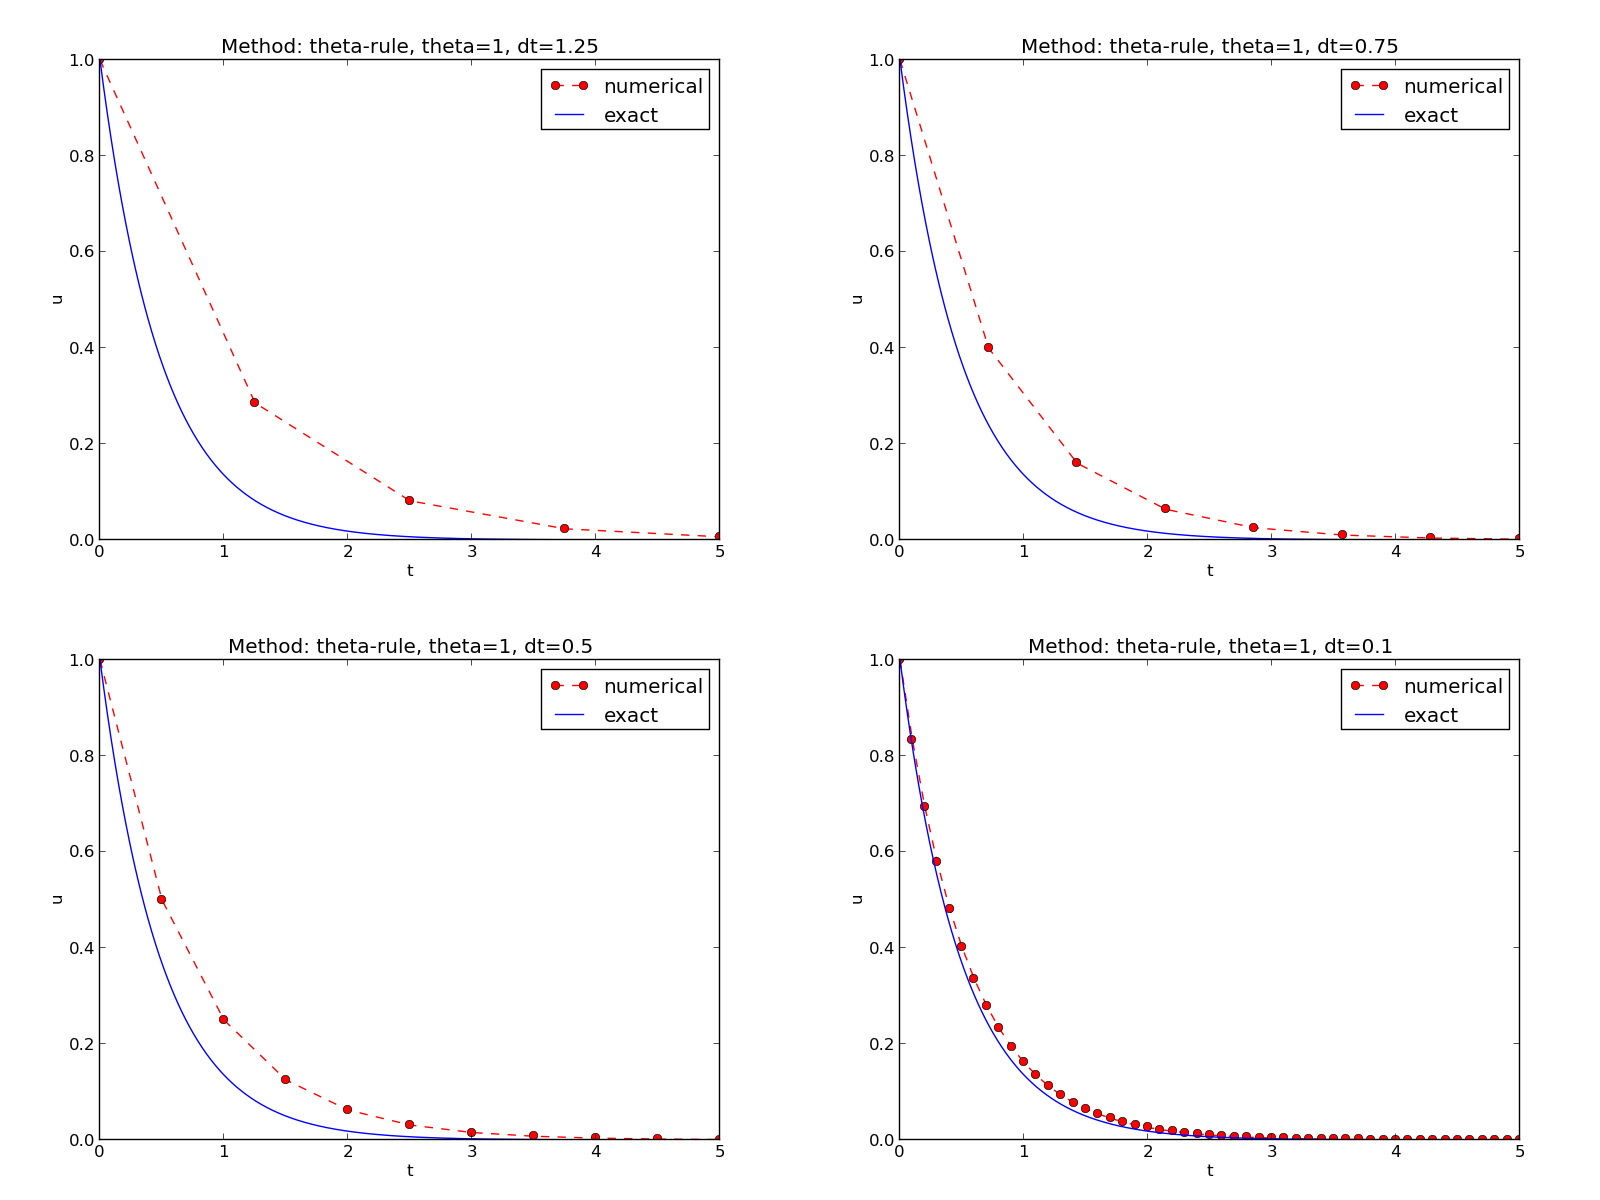
\includegraphics[width=0.9\linewidth]{BE.png}}
\end{center}




% Subsection with inline figure (figure without caption).

\subsection{The Crank-Nicolson method}

\index{CN}


\begin{center}  % inline figure
  \centerline{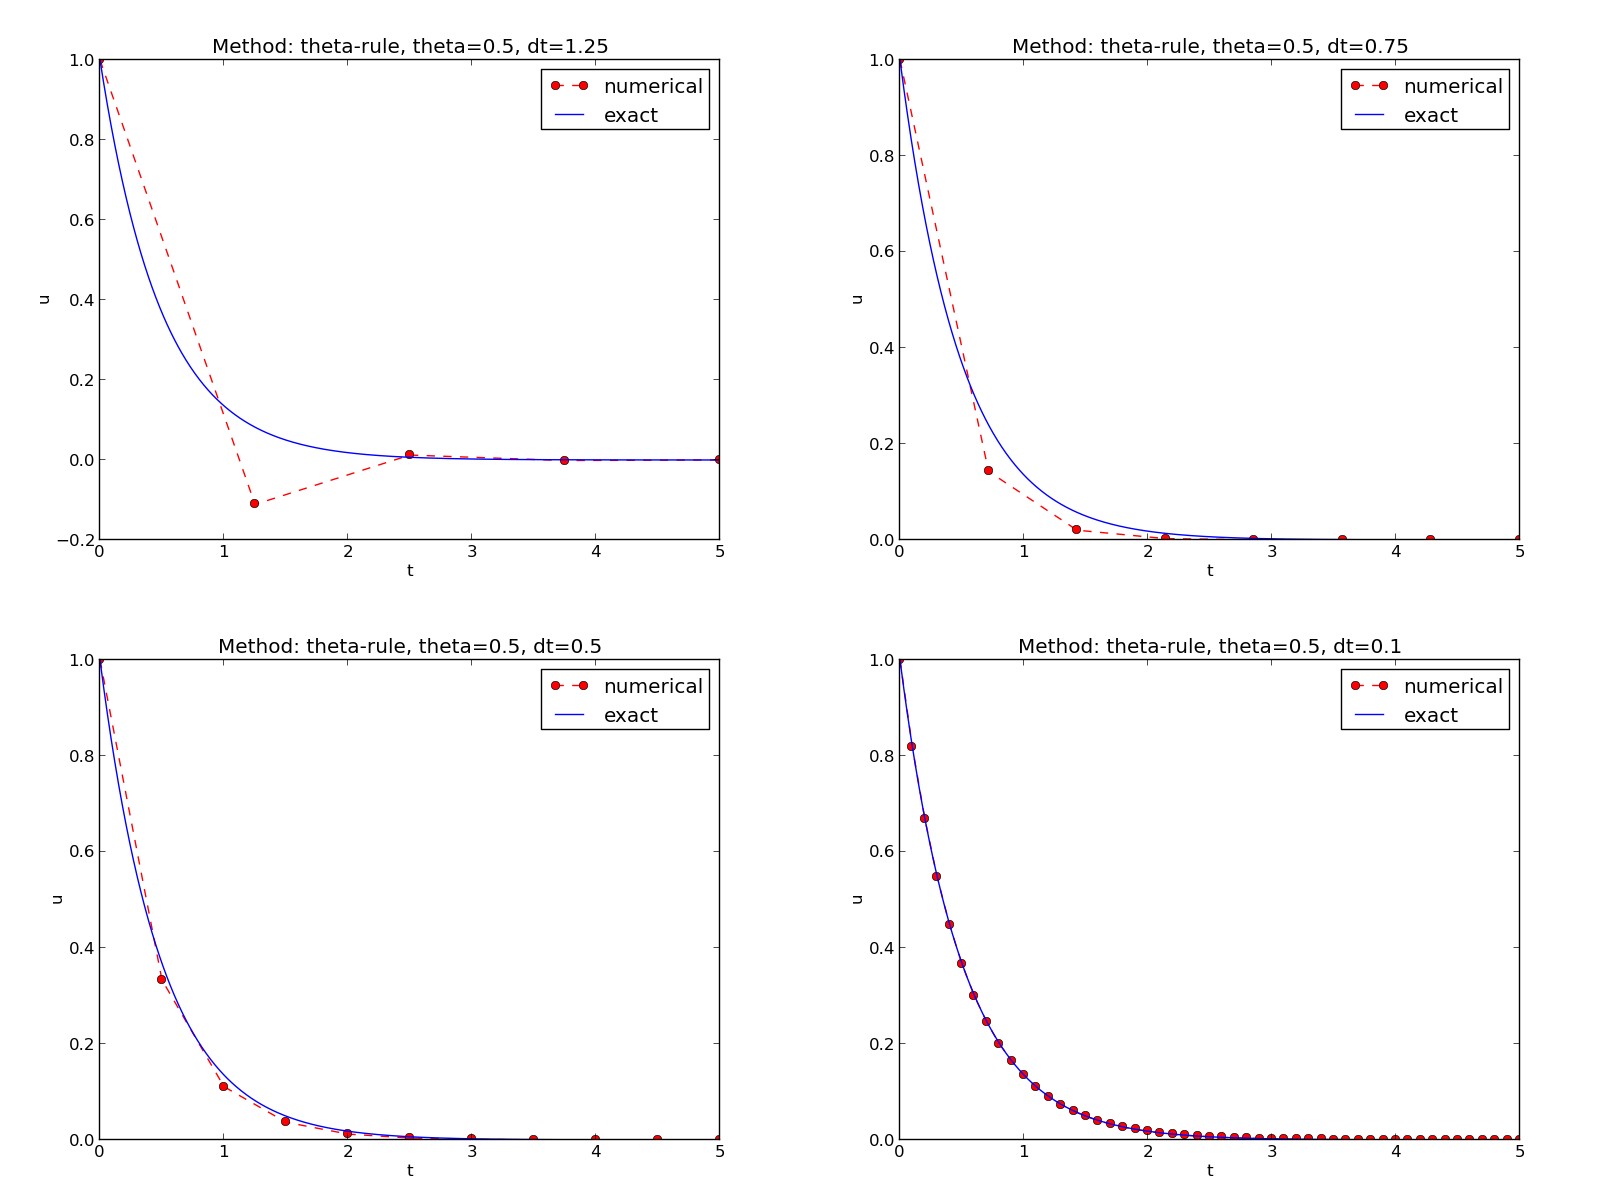
\includegraphics[width=0.9\linewidth]{CN.png}}
\end{center}




% Subsection with inline figure (figure without caption).

\subsection{The Forward Euler method}

\index{FE}


\begin{center}  % inline figure
  \centerline{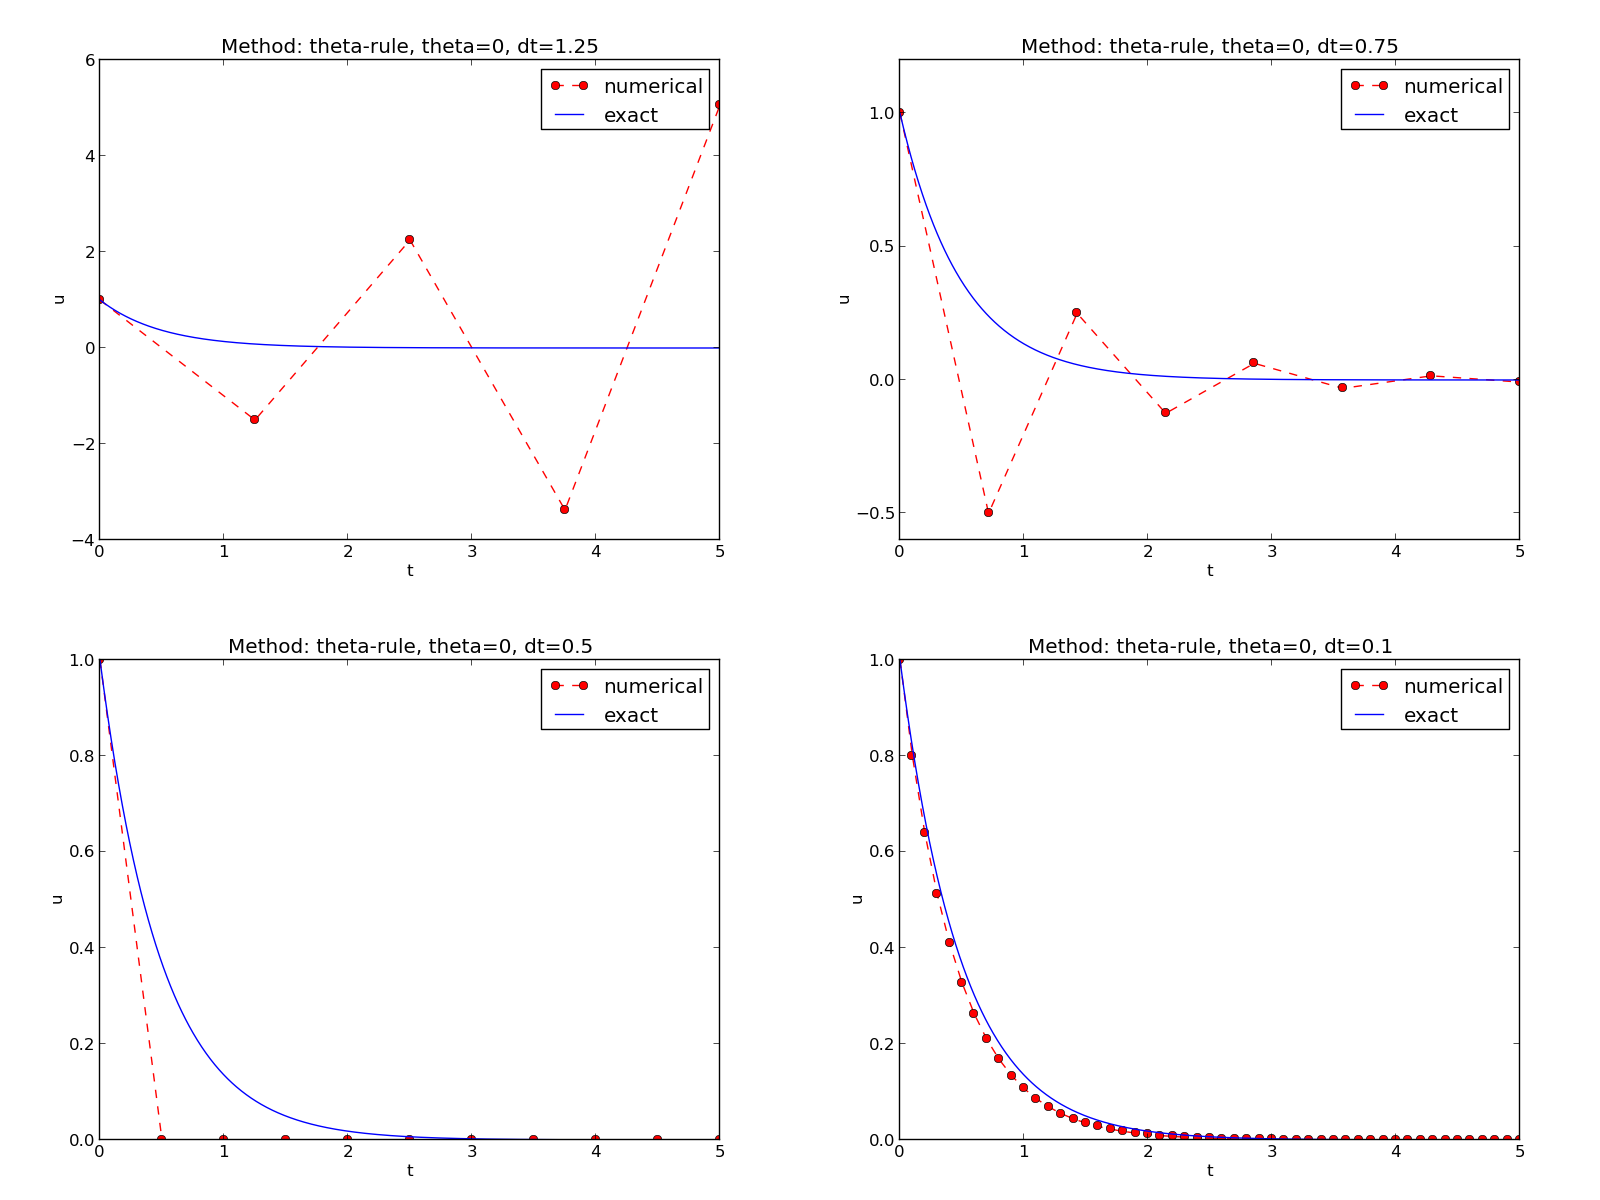
\includegraphics[width=0.9\linewidth]{FE.png}}
\end{center}

\subsection{Error vs $\Delta t$}

% Exemplify referring to a figure with label and caption.

\index{error vs time step}

How $E$ varies with $\Delta t$ for $\theta=0,0.5,1$
is shown in Figure~\ref{fig:E}.


\begin{figure}[!ht]
  \centerline{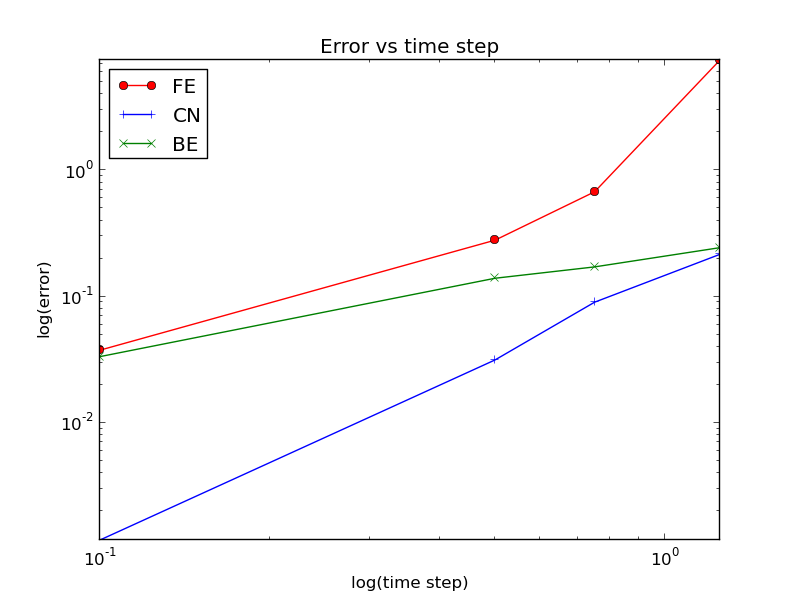
\includegraphics[width=0.9\linewidth]{error.png}}
  \caption{
  Error versus time step. \label{fig:E}
  }
\end{figure}
%\clearpage % flush figures fig:E

\printindex

\end{document}
